\documentclass[tikz, border=0mm, convert={density=300,size=1080x800, outext=.png}]{standalone}
\usepackage{amsmath}
\usepackage[most]{tcolorbox}
\usetikzlibrary{backgrounds}

\begin{document}
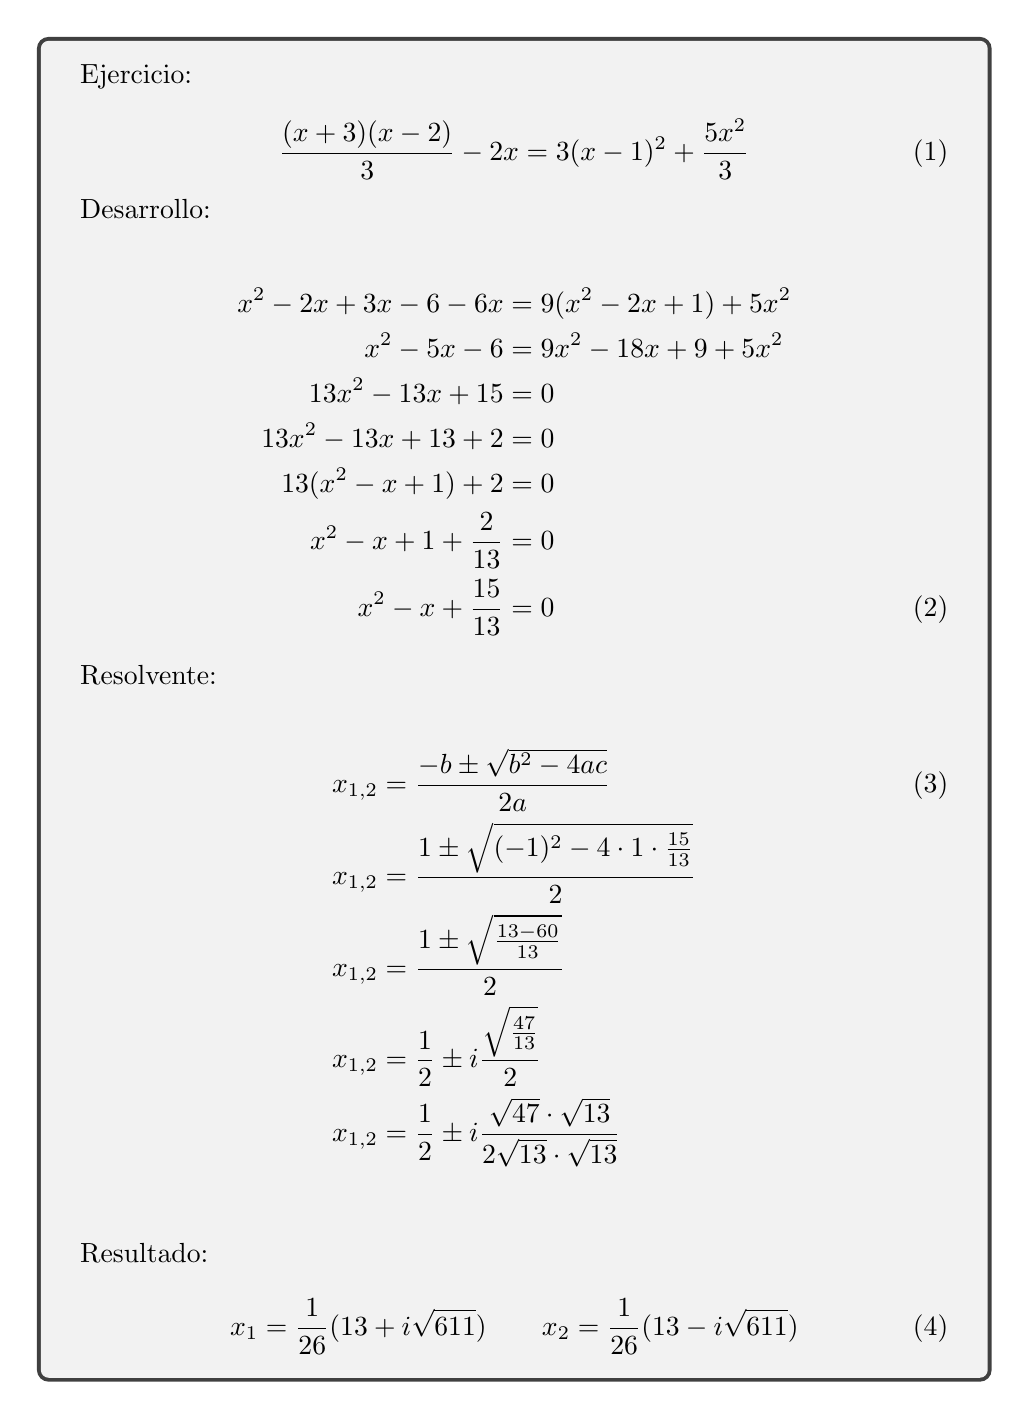
\begin{tikzpicture}[auto]
\node at (0,0) {%
\begin{tcolorbox}
    Ejercicio:
    
    \begin{equation}
        \frac{(x+3)(x-2)}{3} -2x = 3(x-1)^2 + \frac{5x^2}{3}
    \end{equation}
        
    Desarrollo:
    
    \begin{align*}
        x^2 - 2x + 3x - 6 -6x &= 9(x^2 -2x +1) + 5x^2\\ 
        x^2 -5x -6 &= 9x^2 -18x +9 +5x^2 \\ 
        13x^2 -13x + 15 &= 0 \\
        13x^2 -13x + 13 + 2 &= 0 \\
        13(x^2 -x + 1) + 2 &= 0 \\
        x^2 -x + 1 + \frac{2}{13} &= 0 \\
        x^2 -x  + \frac{15}{13} &= 0 \tag{2}
    \end{align*}

    Resolvente:

    \begin{align*}
        x_{1, 2} &= \frac{-b \pm \sqrt{b^2 - 4ac}}{2a} \tag{3}\\
        x_{1, 2} &= \frac{1 \pm \sqrt{(-1)^2 - 4\cdot 1 \cdot \frac{15}{13}}}{2}\\
        x_{1, 2} &= \frac{1 \pm \sqrt{\frac{13 - 60}{13}}}{2}\\
        x_{1, 2} &= \frac{1}{2} \pm i\frac{\sqrt{\frac{47}{13}}}{2}\\
        x_{1, 2} &= \frac{1}{2} \pm i\frac{\sqrt{47}\cdot \sqrt{13}}{2 \sqrt{13}\cdot \sqrt{13}}\\
    \end{align*}

    Resultado:

    \begin{equation*}
        x_1 = \frac{1}{26}(13 + i\sqrt{611}) \qquad x_2 = \frac{1}{26}(13 - i\sqrt{611})\tag{4}
    \end{equation*}
\end{tcolorbox}
};
\end{tikzpicture}
\end{document}